\section{Booleova algebra}
-kombinační obvody (úplně určená funkce více proměnných) x sekvenční obvody (stavové automaty Mealy, Moor
\subsection{Boolova algebra}
V Booleově algebře se používají logické
reprezentace dvouhodnotových veličin - logických
proměnných.

Základní zákony této algebry mají podobný tvar
jako mají zákony běžné algebry.

Hodnota logického výrazu s operátory logického
součtu a logického součinu se nezmění, jestliže
vzájemně tyto operátory zaměníme (tj. operátory
logického součtu nahradíme operátory logického
součinu a naopak), invertujeme proměnné
a výsledek.
   \begin{figure}[h]
   \begin{center}
     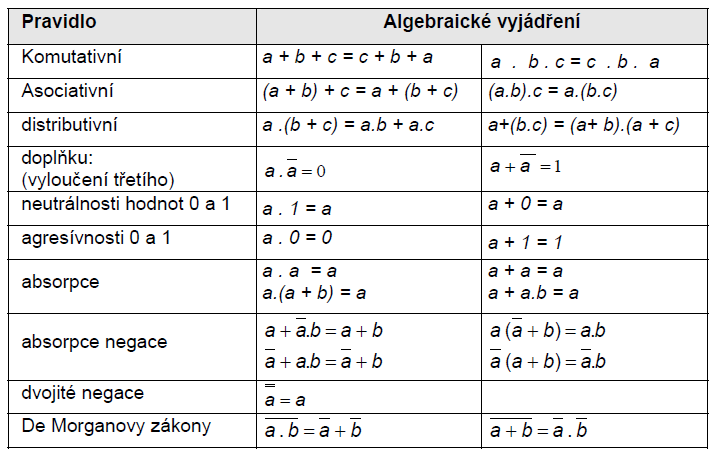
\includegraphics[scale=0.6]{images/Bool.png}
   \end{center}
   \caption{Boolova algebra}
  \end{figure}


\textbf{Z de Morganových pravidel plyne:}\\
Součtový term sestavený z určité kombinace vstupních proměnných je
roven inverzi součinového termu sestaveného z týchž proměnných, které
mají opačné znaky inverze, tj. proměnná obsažená v součtovém termu
bez inverze je v odpovídajícím součinovém termu invertovaná
a naopak.

\subsection{Kombinační vs. sekvenční obvody}
\textbf{Kombinační}\\
Výstupní stav závisí pouze na okamžitých stavech (kombinacích) vstupních logických proměnných\\

\textbf{Sekvenční}\\
Hodnoty výstupní proměnných sekvenčních logických obvodů jsou dány nejen
současnými hodnotami vstupních logických proměnných, ale také minulými hodnotami
vstupních logických proměnných. Informace o historii (minulých hodnotách vstupních
logických proměnných) jsou dány vnitřním stavem sekvenčního logického obvodu, tj. jeho
hodnotami jeho stavových logických proměnných. Hodnoty stavových proměnných jsou
uchovávány v paměťových členech, v praxi realizovaných pomocí klopných obvodů.
Sekvenční logické obvody dělíme na asynchronní a synchronní.


\subsection{Kombinační obvody}
Abychom mohli s kombinačními logickými funkcemi
pracovat, musíme je nejprve zapsat či zobrazit.\\
Nejčastěji se používají tyto způsoby zápisu, popř.
zobrazení kombinačních logických funkcí:
\begin{itemize}
\item zápis pomocí pravdivostní tabulky,
\item zápis logickým výrazem,
\item zobrazení pomocí mapy,
\item zobrazení pomocí logického schématu.
\end{itemize}

   \begin{figure}[h]
   \begin{center}
     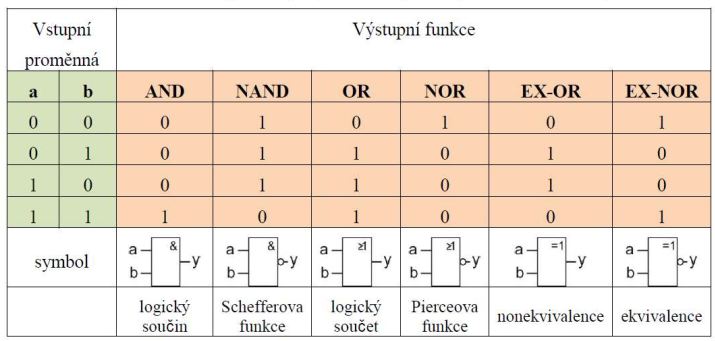
\includegraphics[scale=0.6]{images/Tab.png}
   \end{center}
   \caption{Zápis nejdůležitějších logických funkcí v prav. tabulce}
  \end{figure}

Různé způsoby a s použitím různých operátorů.\\
Dva základní způsoby zápisu funkce:\\
\textbf{1. Součet součinů (Sum of Products, SOP)}\\
Nazývá se také AOI (AND-OR-INVERTOR)\\
Pro úplné termy (= mintermy) - úplný součtový tvar zápisu\\
Pro některé neúplné termy - zkrácený (zjednodušený) součtový tvar zápisu.\\

\textbf{2. Součin součtů (Product of Sums, POS})\\
Nazývá se také OAI (OR-AND-INVERTOR)\\
Pro úplné termy (= maxtermy) - úplný součinový tvar zápisu\\
Pro některé neúplné termy - zkrácený (zjednodušený) součinový tvar zápisu.\\

   \begin{figure}[h]
   \begin{center}
     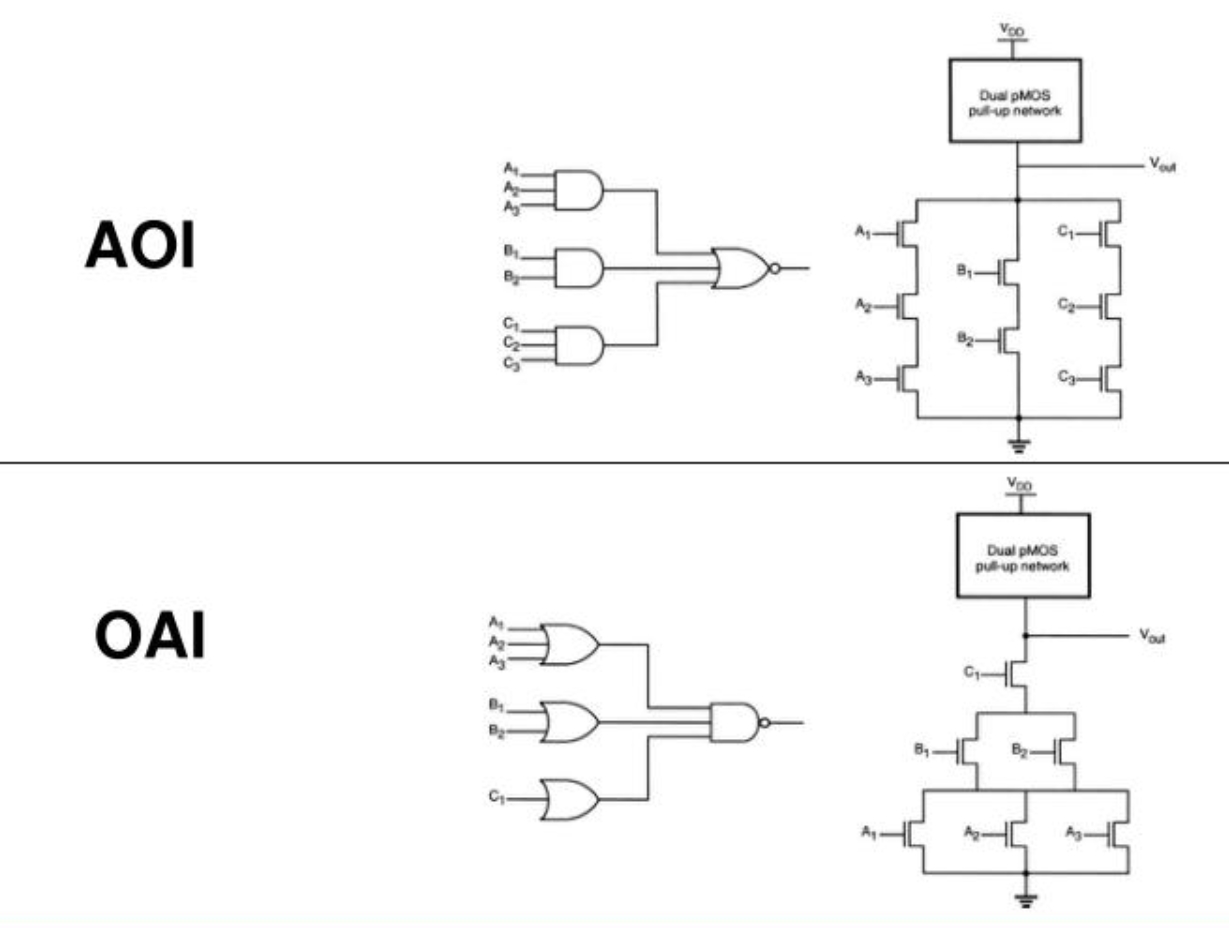
\includegraphics[scale=0.3]{images/AOI.png}
   \end{center}
   \caption{AOI vs. OAI}
  \end{figure}
  
   \begin{figure}[h]
   \begin{center}
     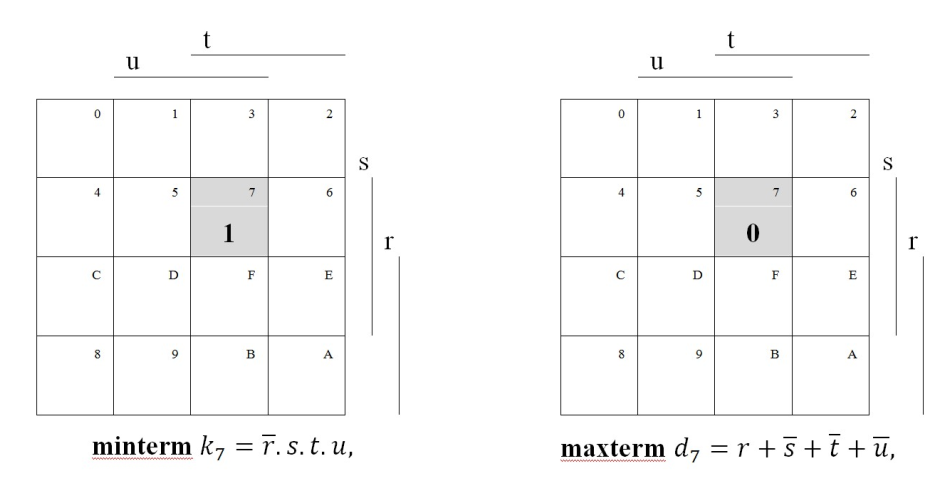
\includegraphics[scale=0.6]{images/minterm.png}
   \end{center}
   \caption{Minterm a Maxterm}
  \end{figure}  

Zápis funkce v úplném součtovém a součinovém tvaru je
jednoznačný. Minimálních tvarů však může být pro určitou funkci více.
Někdy může být potřebné doplnit zkrácený tvar zápisu logické funkce na
úplný tvar. Bývá to například při realizaci funkcí pomocí multiplexorů. Úpravu je možno
provést tak, že se členy, které neobsahují některé proměnné, doplní činiteli typu (a+not(a)), kde a je proměnná chybějící v členu.

Realizace kombinační logické funkce = sestavení zapojení
obvodu, který ze vstupních proměnných vytvoří výstupní
proměnné v souhlasu se zadanou logickou funkcí.

Použití moderních mikroelektronických součástek
často stačí jediný IO (katalog nebo PROM nebo PLD)

Základní způsob realizace kombinační logické funkce =
pomocí kombinačních logických obvodů představujících
realizaci základních logických členů v integrované podobě,
kdy se vychází ze zápisu logické funkce v některém z výše
uvedených tvarů součtu součinů nebo součinu součtů.

\subsection{Sekvenční obvody}
\subsubsection{Asynhronní}
Nejjednodušším klopným obvodem je klopný obvod RS (Reset – nulování, Set -
nastavení). Od RS klopného obvodu jsou odvozeny ostatní typy klopných obvodů jako JK, D
a T.
   \begin{figure}[h]
   \begin{center}
     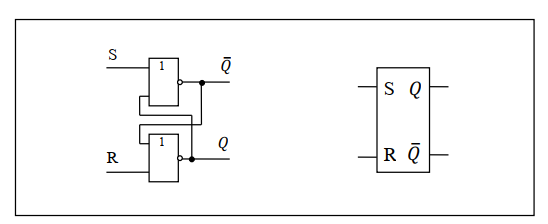
\includegraphics[scale=0.6]{images/RS.png}
   \end{center}
   \caption{RS KO realizovaný pomocí NOR hradel}
  \end{figure}
   \begin{figure}[h]
   \begin{center}
     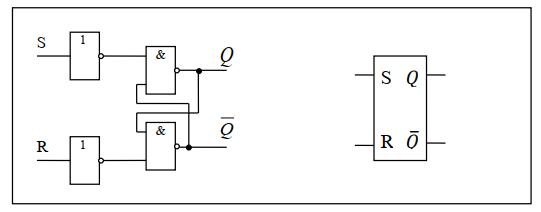
\includegraphics[scale=0.6]{images/RSNAND.png}
   \end{center}
   \caption{RS KO realizovaný pomocí NAND hradel}
  \end{figure}

\subsubsection{Synhronní}
\subsubsection*{RS}
Upravený klopný obvod RS synchronizovaný impulsy na hodinovém
vstupu C. Je-li hodinový signál na úrovni logické 0, klopný obvod si pamatuje dříve
nastavený stav. Při úrovni logické 1 na hodinovém vstupu se mění stav klopného obvodu
(logické úrovně na výstupu Q resp. notQ ) dle pravdivostní tabulky klopného obvodu. Hladinové klopné obvody bývají v anglické literatuře označovány jako \textbf{latch}.
   \begin{figure}[h]
   \begin{center}
     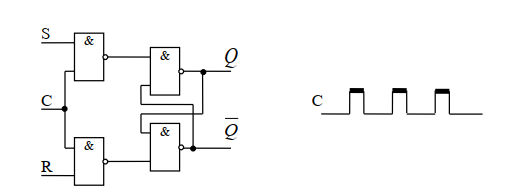
\includegraphics[scale=0.6]{images/RSsynch.png}
   \end{center}
   \caption{Synchronní RS KO}
  \end{figure}

\subsubsection*{D}
  Dalším používaným typem klopných je klopný obvod D (Data). Klopný obvod D kopíruje při příchodu synchronizačního impulsu.
   \begin{figure}[h]
   \begin{center}
     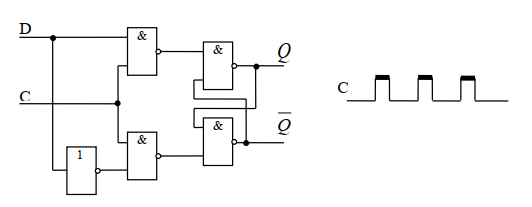
\includegraphics[scale=0.6]{images/D.png}
   \end{center}
   \caption{D KO}
  \end{figure}  

\subsubsection*{JK}
JK klopný obvod odstraňuje problém RS klopného obvodu se zakázanými přechody
mezi kombinacemi vstupních signálů.
   \begin{figure}[h]
   \begin{center}
     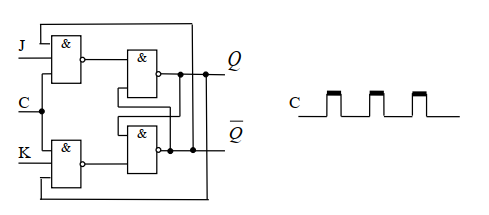
\includegraphics[scale=0.6]{images/JK.png}
   \end{center}
   \caption{JK KO}
  \end{figure} 



\subsection{Stavové automaty}
Rozlišujeme stavové automaty Moorova a Mealyho typu. 
U stavového automatu \textbf{Moorova} typu závisí výstupní signály pouze na stavu automatu.\\
U stavového automatu \textbf{Mealyho} typu závisí výstupní signál i na vstupních signálech.\\
   \begin{figure}[h]
   \begin{center}
     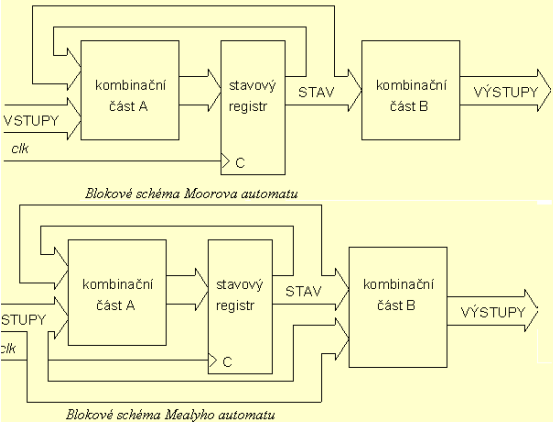
\includegraphics[scale=0.6]{images/Moor.png}
   \end{center}
   \caption{Stavové automaty}
  \end{figure}  



















